\chapter{Method} \label{cha:method}

This study is carried out in two stages: \textit{identification}, where attention heads are identified; and \textit{ablation} where the output of the selected attention heads outputs are intentionally set to 0 and compared to a clean run baseline and random ablation conditions. The structure of this section is as follows: Section \ref{sec:data} starts with describing the dataset used, as well as how it was preprocessed and filtered. Section \ref{sec:identification} goes through the identification of attention heads and the Section \ref{sec:ablation} the ablation methodology.

\section{Data}\label{sec:data}

The analysis is performed on Chinese, English and Turkish using the Universal Dependencies PUD (UD-PUD) treebanks \citep{nivre2020, akhundjanova2025}, a multilingual corpus derived from Wikipedia and news articles. The data breakdown is presented in Table~\ref{tab:databreakdown}. UD-PUD contains parallel sentences annotated with syntactic dependencies. The parallel nature of the corpus allows comparing attention behavior across languages while minimizing domain differences. Throughout the thesis, a word will correspond to a syntactic word as annotated in UD, providing a cross-lingually consistent unit without introducing tokenizer-specific assumptions.

\begin{table}[ht]
\small
\centering
\begin{tabular}{lrrrr}
\toprule
& \textbf{Sequences} & \textbf{Tokens} & \textbf{Multi-token words} & \textbf{Non-space words}\\
\midrule
English & 1000 & 21051 & 129 & 2621 \\
Chinese & 1000 & 21415 & 0 & 20322 \\
Turkish & 1000 & 16535 & 346 & 2179 \\
\bottomrule
\end{tabular}
\caption[Parallel Universal-Dependencies Breakdown]{Parallel Universal-Dependencies data breakdown; Multi-token words include UD-words such as `it's', `that's', `city's'}
\label{tab:databreakdown}
\end{table}


To avoid trivial cross-lingual matches, words with part-of-speech tags that often remain unchanged across languages are excluded, including punctuation, proper nouns, symbols, and numbers. Tokens are discarded which occur before the fourth position in a sequence, as limited preceding context and positional effects (e.g., the first token acting as an attention sink \citep{xiao2024efficient}) can confound the analysis. After filtering, the data is randomly shuffled and 250 unique words are sampled with their preceding context for each language and configuration.

\section{Identification}\label{sec:identification}

A key challenge is that tokenization efficiency varies substantially across languages and tokenizers, making simple distinctions such as single-token vs. multi-token words used in \citet{kaplan2025} non-comparable. For example, under the GPT-2 tokenizer, which is not trained on Chinese, most Chinese words span multiple tokens due to their higher byte length. As a result, a ``single-token word'' in Chinese is not comparable to one in English or Turkish, which is further amplified in byte-level tokenizers. To address this, boundary-based conditions inspired by \citet{kaplan2025, ferrando2024informationflow} are used. The in-boundary condition measures attention from the final subtoken of a word to its penultimate subtoken, while the out-boundary condition measures attention from the first subtoken of a word to the final subtoken of the preceding word. See Figure~\ref{fig:boundary_example} for an example.

\begin{figure}[ht]
\centering

\begin{subfigure}{0.45\textwidth}
\centering
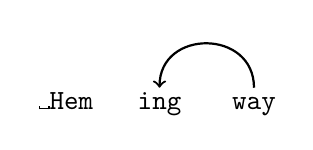
\begin{tikzpicture}[baseline, every node/.style={text height=1ex, text depth=.25ex}, node distance=1.2cm]
\node (1) {\texttt{␣Hem}};
\node (2) [right of=1] {\texttt{ing}};
\node (3) [right of=2] {\texttt{way}};
\draw[->, thick] (3.north) to[out=90,in=90,looseness=1.6] (2.north);
\end{tikzpicture}
\caption{in-boundary}
\end{subfigure}
\hfill
\begin{subfigure}{0.45\textwidth}
\centering
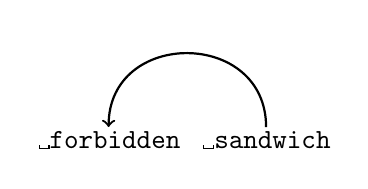
\begin{tikzpicture}[baseline, every node/.style={text height=1ex, text depth=.25ex}, node distance=2cm]
\node (1) {\texttt{␣forbidden}};
\node (2) [right of=1] {\texttt{␣sandwich}};
\draw[->, thick] (2.north) to[out=90,in=90,looseness=1.6] (1.north);
\end{tikzpicture}
\caption{out-boundary}
\end{subfigure}

\caption[Boundary condition examples]{Examples of each condition in GPT-2: in-boundary (left) and out-boundary (right). Arrows denote attention from a source token to a target token.}
\label{fig:boundary_example}
\end{figure}


The setup follows the hypothesis proposed by \citet{kaplan2025, ferrando2024informationflow}. If information about a word's internal structure is propagated through the residual stream, and specific attention heads are involved in aggregating subword units, then such heads should preferentially attend from the final subtoken of a word to preceding subtokens within the same word. Under this hypothesis, attention from the final subtoken to the penultimate subtoken should be stronger than attention that crosses a word boundary. The out-boundary condition serves as a control.

For each layer $l$ and head $h$, the mean attention weight under each condition is calculated across all eligible tokens as described in Section~\ref{sec:data}. The attention weight delta is then defined as:
\begin{equation}\label{eq:delta_attn}
\Delta^{(\text{attn})}_{l,h} = \mu_{l,h}^{(\text{in})} - \mu_{l,h}^{(\text{out})}.
\end{equation}

However, as noted by \citet{jain2019, serrano2019}, attention weights alone may not reflect a head's \textit{contribution} to downstream representations. Following \citet{kobayashi2020}, the magnitude of the attention output is also considered. Specifically, for each head its output is extracted prior to the output projection (i.e.\ before head mixing) and its vector norm is then computed. We then define the corresponding norm delta:
\begin{equation}\label{eq:delta_norm}
\Delta^{(\text{norm})}_{l,h} = \mu_{l,h}^{(|\text{in}|)} - \mu_{l,h}^{(|\text{out}|)}.
\end{equation}

The score to identify candidate heads is then the sum of the $z$-normalized norm/weight deltas:
\begin{equation}\label{eq:headscore}
S_{l,h} = z^{(\text{attn})}_{l,h} + z^{(\text{norm})}_{l,h}
\end{equation}

\section{Ablation}\label{sec:ablation}

For \textbf{RQ2}, patterns are evaluated using the TokSuite models \citep{altintas2025}, a family of 1B Llama-2–style models trained on the same amount of tokens across five languages: 40B tokens for English and 15B tokens each for Turkish, Chinese, Italian, and Farsi. The models share architecture and data distribution, differing only in tokenizer and effective training volume in bytes, since token counts are not directly comparable across tokenizers. To probe tokenizer effects, representative designs are selected: the GPT-2 tokenizer \citep{radford2019} (English-centric BPE), the Aya tokenizer \citep{aya} (large vocab, multilingual BPE), the XGLM-564M tokenizer \citep{xglm} (Unigram with byte fallback), and the ByT5 tokenizer \citep{xue2022} (byte-level). To examine scaling (RQ3), Qwen2.5 models are used\citep{qwen2.5, qwen2}, spanning 0.5B to 7B parameters across 29 languages\footnote{The exact training data composition is not publicly available.}. In the rest of the text, the models will be refered to by their shorthand; e.g.\ ``Toksuite model with XGLM-564M tokenizer'' $\rightarrow$ \texttt{xglm} for brevity.

Bytes per token (BPT), $BPT = \frac{\text{tokens}}{\text{bytes}}$, along with vocabulary size, are reported in Table~\ref{tab:fertility} to capture tokenizer differences.

\begin{table}[ht]
\small
\centering
\begin{tabular}{l c ccc}
\toprule
& & \multicolumn{3}{c}{\textbf{BPT Score}} \\
\cmidrule(lr){3-5}
\textbf{Tokenizer} & \textbf{Vocab size} & \textbf{English} & \textbf{Turkish} & \textbf{Chinese} \\
\midrule
\texttt{aya} & 255k & 4.68 & 4.35 & 4.05 \\
\texttt{byt5} & 256 & 1.00 & 1.00 & 1.00 \\
\texttt{gpt2} & 50k & 4.63 & 2.30 & 1.36 \\
\texttt{qwen2.5} & 151k & 4.52 & 3.17 & 3.67 \\
\texttt{xglm} & 256k & 4.59 & 4.47 & 3.38 \\
\bottomrule
\end{tabular}
\caption[Tokenizer statistics over UD-PUD]{Tokenizer statistics over UD-PUD: vocabulary size and byte/token (BPT) scores for English, Turkish, and Chinese. Higher BPT indicates better per-byte compression.}
\label{tab:fertility}
\end{table}


The aim is to evaluate whether candidate attention heads contribute to representations useful for word reconstruction. To do this, zero-ablation \citep{michel2019}, which removes selected heads by setting their outputs to zero, is combined with Patchscopes \citep{ghandeharioun2024}, an activation patching method \citep{vig2020}. Patchscopes extracts a hidden state from a source forward pass (at a given layer and token position) and inserts it into a separate forward pass on a target prompt designed to elicit specific information.

Following \citet{kaplan2025}, this is framed as a word retrieval task. Given a multi-token word and its preceding context, reconstruction accuracy of the full word from the final-token representation is measured. The prompt \texttt{"Repeat the following word: X, X, X,"} is used, where \texttt{X} is replaced by the patched representation. The prompt is translated into Chinese\footnote{\texttt{重复这个词语：X、X、X、}} and Turkish\footnote{\texttt{Bu kelimeyi tekrarla: X, X, X,}} by native speakers. Under the detokenization hypothesis, retrieval accuracy should be higher in lower layers, where full-word representations are reconstructed. If specific attention heads implement this mechanism as part of a staged inference process, then targeted ablation should impair retrieval, whereas random ablation should have minimal effect.

Three conditions are evaluated:

\begin{enumerate}
\tightlist
\item No ablation
\item Targeted ablation removing the top 1/3/5\% highest-scoring attention heads (Equation~\ref{eq:headscore})
\item Random ablation of \textbf{an equal number} of heads from the same layers as the targeted ablation.
\end{enumerate}

Ablation is capped at 50\% of heads per layer to maintain a valid control. Candidate heads are identified separately for each model/language pair, and is only picked from the first fifteen layers since \textit{detokenization} is hypothesized to be an early-layer phenomena. For each condition, Patchscopes is applied and retrieval performance measured.

Due to computational constraints, reconstruction is only performed from the hidden state output, rather than additionally probing the FFN as in \citet{kaplan2025}.
